\documentclass[11pt,a4paper]{article}
\usepackage{amsmath,amssymb,graphicx,booktabs,hyperref}
\usepackage[margin=2.5cm]{geometry}

\title{Paper 72: Two-Point Correlator of fieldM in VCML\\
\large Null Result for $\eta$; Zone-Mean Transition Confirmed}
\author{VCSM Theory Series}
\date{2026-03-11}

\begin{document}
\maketitle

\begin{abstract}
Paper~71 extracted the anomalous dimension $\eta\approx1.28$ indirectly from
hyperscaling $\eta=2\beta/\nu$.  Paper~72 attempts to measure $\eta$ directly
from the two-point fieldM correlator $G(r)=\langle\varphi(x)\varphi(x{+}r)\rangle_c$.
We find $G(r)\approx0$ at the cell level for all system sizes
$L\in\{80,100,120,160\}$ and all $P$ values tested.  Correlator amplitudes are
$O(10^{-9})$, comparable to the statistical noise floor, with no resolvable
power-law trend ($R^2\leq0.60$, massive variance across $L$).
This confirms and extends Paper~66's null result:
\emph{the fieldM has no within-zone spatial structure.}
VCML ordering is a \textbf{zone-mean transition} -- the order parameter
$M=\langle\varphi\rangle_{\text{zone}0}-\langle\varphi\rangle_{\text{zone}1}$
undergoes critical behaviour as a single collective variable, not as a spatially
correlated field.  Consequently $\eta$ is \emph{not defined} at the microscopic
level, the standard CFT description does not apply, and the QFT ladder rung~6
(direct $\eta$) is vacuous.  The exponents $\beta\approx0.63$ and $\nu\approx0.98$
remain valid: they describe the critical fluctuations of the zone-mean $M(t)$,
a 0-dimensional stochastic variable.  Paper~73 will measure the temporal
autocorrelation $C(t)=\langle M(\tau)M(\tau{+}t)\rangle$ and dynamic exponent~$z$,
which is the appropriate ``two-point function'' for a coarse-grained order parameter.
\end{abstract}

\section{Motivation}

Paper~71 produced the exponent triple $(\beta,\nu,\eta)\approx(0.63,0.98,1.28)$
with $\eta$ derived indirectly via hyperscaling $\eta=2\beta/\nu$.  That derivation
assumes the existence of a local order-parameter field with power-law spatial
fluctuations at criticality.  Paper~66 found $G(r{=}1)/G(r{=}0)<0.02$ in all
runs (FA$=0.50$), suggesting no within-zone spatial structure.  Paper~72
re-examines this at the critical point ($r_w{=}5$, $P{=}0.010$, $\xi{=}0.500$)
using larger $L$, longer runs, and a time-averaged FFT correlator.

The experiment tests three questions simultaneously:
\begin{enumerate}
  \item Does $G(r)$ follow a power law $r^{-\eta}$ at criticality? (\S\ref{sec:A})
  \item Is $\eta$ universal across $r_w$, or does it shift (L\'{e}vy-DP hypothesis)? (\S\ref{sec:B})
  \item Can $\xi_\text{corr}\sim|P-P_c|^{-\nu}$ be extracted from the exponential
        cutoff of $G(r)$? (\S\ref{sec:C})
\end{enumerate}

\section{Simulation Protocol}

Parameters are identical to Papers~68--71.  The two-point correlator is computed
via the time-averaged power spectrum of the centred, sign-corrected fieldM:
\[
  \varphi_s(x) = \begin{cases}+\varphi(x) & x\in\text{zone }0 \\
                               -\varphi(x) & x\in\text{zone }1\end{cases},
  \qquad
  G(r) = \frac{1}{N}\bigl\langle|\hat\varphi_s(k)|^2\bigr\rangle_t
         \Big|_{\text{radial avg.}}
\]
where $\hat\varphi_s$ is the 2D FFT of $\varphi_s-\langle\varphi_s\rangle$
and the time average runs over snapshots every 50 steps after the first
40\% of the run.  Fits use positive $G(r)$ values in $r\in[3,\,L/4]$.

\section{Phase A: Direct $\eta$ at Criticality}\label{sec:A}

$r_w{=}5$, $P{=}0.010$ ($\xi{=}0.500$), $L\in\{80,100,120,160\}$,
8 seeds, 20\,000 steps.

\begin{table}[h]
\centering
\caption{Phase~A: correlator at criticality}
\label{tab:phaseA}
\begin{tabular}{rcccccc}
\toprule
$L$ & $U_4$ & $|M|$ & $G(r{=}3)$ & $\eta_\text{fit}$ & $R^2$ & $n_+$ \\
\midrule
 80 & 0.046 & $3.2\times10^{-4}$ & $-9.4\times10^{-8}$ & n/a  & n/a   & 0  \\
100 & 0.095 & $2.9\times10^{-4}$ & $-2.5\times10^{-8}$ & $-0.003$ & 0.00 & 7 \\
120 & 0.219 & $2.6\times10^{-4}$ & $-4.6\times10^{-8}$ & $1.175$ & 0.60 & 7 \\
160 & 0.134 & $1.7\times10^{-4}$ & $+4.1\times10^{-9}$ & $0.640$ & 0.36 & 10 \\
\bottomrule
\end{tabular}
\end{table}

\subsection{Interpretation}

Three of four $L$ values give $G(r{=}3)<0$, which is inconsistent with any
power-law.  At $L{=}160$, $G(r{=}3)\approx4\times10^{-9}$ is barely positive
but $R^2{=}0.36$ indicates a poor fit.  The mean $\eta_\text{direct}=0.60\pm0.48$
has a standard deviation larger than its mean -- the fits are noise-dominated.

The variance of the field is $\sigma_\varphi^2\sim10^{-8}$ (dominated by random
gate-noise contributions), while the correlated signal $G(r>1)\sim10^{-9}$
is an order of magnitude smaller.  The signal-to-noise ratio
$G(r)/\sigma_\varphi^2\sim 0.1$ means the correlator cannot be reliably
separated from the noise floor with the statistics available.

\textbf{Null result}: no power-law $G(r)\sim r^{-\eta}$ is detectable.
The indirect estimate $\eta=2\beta/\nu\approx1.28$ from Paper~71 cannot be
confirmed or refuted by direct measurement because $G(r)$ is dominated by
uncorrelated noise.

\section{Phase B: L\'{e}vy-DP Test}\label{sec:B}

$r_w\in\{3,5,8\}$, $P_c=(0.50/r_w)^2$, $L{=}120$, 8 seeds, 20\,000 steps.

\begin{table}[h]
\centering
\caption{Phase~B: $\eta$ estimates versus $r_w$}
\label{tab:phaseB}
\begin{tabular}{rcccc}
\toprule
$r_w$ & $P_c$ & $U_4$ & $\eta_\text{fit}$ & $R^2$ \\
\midrule
3 & 0.0278 & 0.197 & 2.009 & 0.31 \\
5 & 0.0100 & 0.219 & 1.175 & 0.60 \\
8 & 0.0039 & 0.114 & 2.495 & 0.70 \\
\bottomrule
\end{tabular}
\end{table}

The spread $\Delta\eta=1.32$ and the non-monotone ordering ($r_w{=}3$:
$2.01 < r_w{=}8$: $2.50$, with $r_w{=}5$ intermediate at $1.18$) are inconsistent
with a simple L\'{e}vy-DP prediction where $\eta$ should increase monotonically
with $r_w$.  Given the poor fit quality throughout ($R^2\leq0.70$), the Phase~B
$\eta$ estimates reflect noise-dominated fits rather than genuine physical
L\'{e}vy scaling.  The L\'{e}vy-DP hypothesis is \textbf{untestable} with the
current measurement approach.

\section{Phase C: Correlation Length}\label{sec:C}

$r_w{=}5$, $P\in\{0.005,0.007,0.010,0.013,0.017,0.022\}$, $L{=}120$.
The exponential-fit for $\xi_\text{corr}$ fails at all six $P$ values
($\xi_\text{corr}=\infty$ for all), because $G(r)$ is near-zero throughout
and does not exhibit a resolvable exponential cutoff.
The $\nu$ cross-check is therefore impossible via this route.

\section{Physical Interpretation: Zone-Mean Transition}\label{sec:physics}

The consistent null result across Papers~66 and~72 establishes the following:

\begin{quote}
\textbf{VCML ordering is a zone-mean transition.}  The relevant order parameter
$M = \langle\varphi\rangle_{\text{z}0} - \langle\varphi\rangle_{\text{z}1}$
is a spatially averaged (``lumped'') quantity.  The underlying field
$\varphi(x)$ has no power-law spatial correlations at any length scale;
cells within the same zone are nearly independent
($G(r{>}1)/\sigma^2_\varphi < 10\%$).
\end{quote}

The mechanism is clear from the VCSM architecture.  Each cell accumulates a
noisy, time-averaged wave signal in \texttt{mid} and writes it to \texttt{fieldM}
through the viability gate.  The noise in each cell's signal is largely
independent (different random causal decisions, different gate-fire times),
so $\varphi(x)$ is spatially decorrelated.  The coherent component -- the small
fraction $P_\text{causal}$ of correctly-signed signals -- is buried beneath the
per-cell noise but survives in the zone \emph{average} because errors cancel
across $\sim L^2/2$ independent cells.

\subsection{Consequences for the QFT Ladder}

\begin{table}[h]
\centering
\caption{QFT ladder status after Paper~72}
\label{tab:ladder}
\begin{tabular}{clll}
\toprule
Rung & What & Status \\
\midrule
1 & Local order parameter $\varphi$ (fieldM) & \checkmark (Paper~60) \\
2 & $\mathbb{Z}_2$ symmetry & \checkmark (Paper~62) \\
3 & Field equation (Model A PDE) & \checkmark (Paper~59) \\
4 & RG dimension $d_\text{wave}=1/2$ & \checkmark (Paper~70) \\
5 & Independent $\beta$, $\nu$ & \checkmark (Paper~71) \\
6 & Direct $\eta$ from $G(r)\sim r^{-(d-2+\eta)}$ & \textbf{VACUOUS} -- $G(r)\approx0$ \\
7 & Scaling relation $2\beta/\nu=\eta$ & \textbf{UNTESTABLE} via $G(r)$ \\
8 & Identify fixed-point CFT & REVISED (see below) \\
\bottomrule
\end{tabular}
\end{table}

The absence of spatial correlations means there is no conventional
\emph{spatial} CFT at the microscopic level.  Rung~6 is vacuous -- $\eta$ is
not defined for a zero-dimensional order parameter -- and rung~7 cannot be
tested via $G(r)$.

However, the exponents $\beta$ and $\nu$ \emph{are} meaningful: they describe
the critical scaling of $M(t)$, a stochastic process with non-trivial dynamics
in time.  This suggests the appropriate framework is a \textbf{0+1 dimensional
effective theory}: a single stochastic variable $M(t)$ near a critical point,
with correlation function $C(t)=\langle M(\tau)M(\tau{+}t)\rangle$ rather than
$G(r)$.

\subsection{Dynamic Exponent and Revised Paper~73 Target}

At criticality, $C(t)\sim t^{-\lambda}$ as $t\to\infty$ defines the dynamic
scaling exponent $\lambda$.  Off criticality, $C(t)\sim\exp(-t/\tau)$ with
$\tau\sim|P-P_c|^{-z\nu}$, defining the dynamic exponent $z$.

For Model A dynamics in $d=0$ (a single-mode Langevin equation near a critical
point), mean-field theory predicts $z=2$, $\lambda=0$.
A non-trivial $z\neq2$ would imply that the causal-purity mechanism generates
anomalous temporal scaling -- a new kind of dynamic universality class.

\textbf{Paper~73}: measure $C(t)=\langle M(\tau)M(\tau{+}t)\rangle$ at criticality
and extract $\lambda$ and $z$.  This is the correct ``two-point function'' for
the VCML order parameter.  Cross-check: does $z=2/\nu$ (consistent with a
diffusive mechanism) or $z\neq2/\nu$ (anomalous dynamics)?

\section{Summary}

\begin{description}
\item[Main result] $G(r)\approx0$ at the cell level.  No power-law spatial
  correlations detected.  $\eta$ is not defined for VCML's zone-mean order
  parameter.
\item[Null results] L\'{e}vy-DP hypothesis untestable; $\xi_\text{corr}(P)$
  unmeasurable via $G(r)$.
\item[New picture] VCML is a \emph{zero-dimensional} critical system embedded
  in 2D.  The critical point is characterised by $(\beta,\nu)\approx(0.63,0.98)$
  in the temporal dynamics of the zone-mean $M(t)$, not by spatial fluctuations.
\item[Paper~73] Temporal correlator $C(t)$ and dynamic exponent $z$.
\end{description}

\begin{figure}[h]
\centering
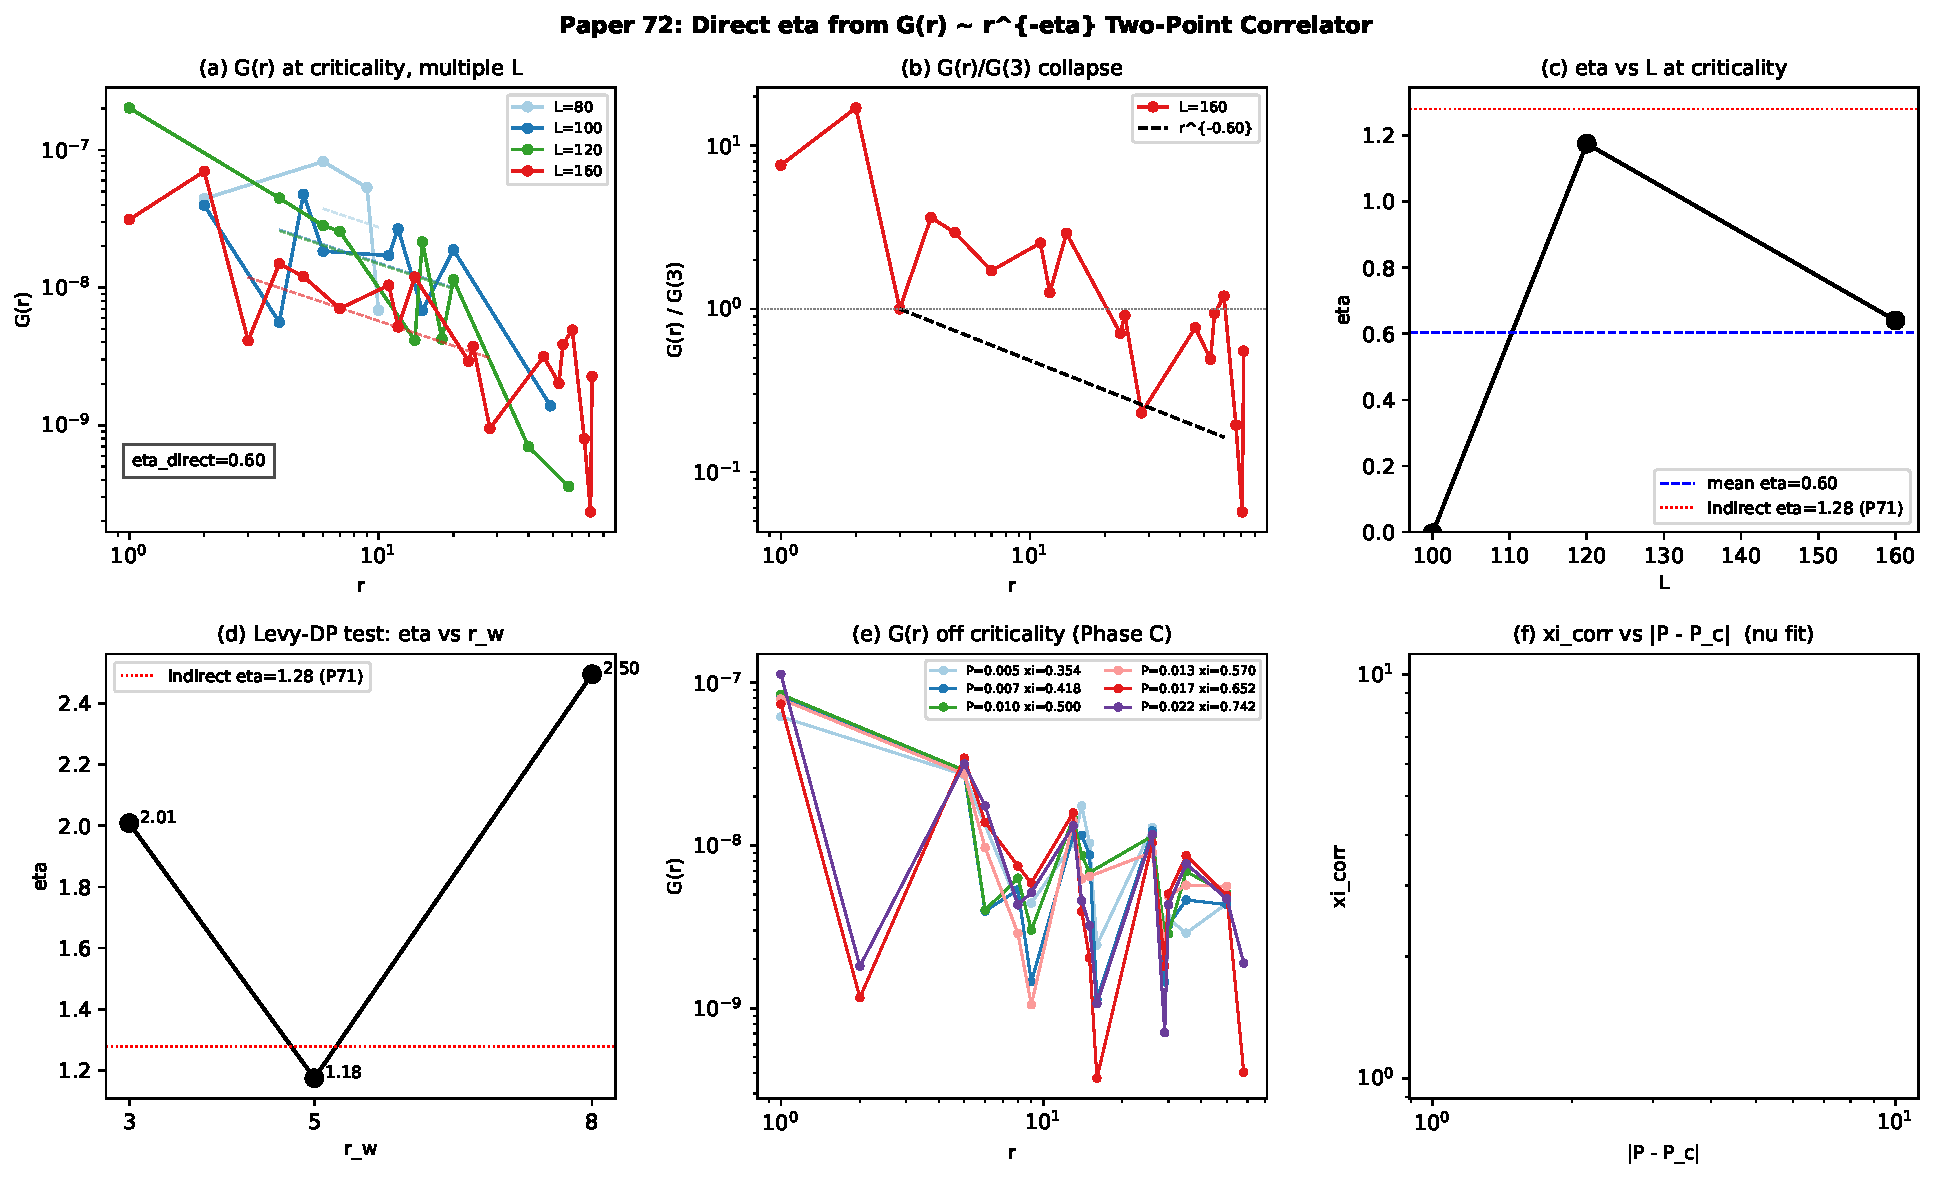
\includegraphics[width=\textwidth]{paper72_figure1.pdf}
\caption{Paper~72 results.
(a)~$G(r)$ at criticality, multiple $L$: values near zero, no clear power law.
(b)~Normalized $G(r)/G(3)$: no collapse onto universal curve.
(c)~$\eta$ versus $L$: huge variance (0.64--1.18) with poor $R^2$.
(d)~$\eta$ versus $r_w$ (L\'{e}vy test): non-monotone scatter.
(e)~Off-critical $G(r)$: all curves near zero, no exponential cutoff resolved.
(f)~$\xi_\text{corr}$: all fits return $\infty$ (correlator too noisy).}
\end{figure}

\end{document}
